\documentclass{article}

\usepackage{graphicx}
\usepackage{epsfig}
%\usepackage{psfig}
%\usepackage{algorithm}
%\usepackage{amsmath, amsthm}
\usepackage{url}

%\setlength{\parindent}{0pt}
%\setlength{\parskip}{10pt}

\begin{document}

\title{Buddy App Documentation	}


\author{
Duy Nguyen
\and
Feng Ji
\and
Zhichao Li
\and
Moussa Ehsan
}

\maketitle

\section{Introduction}
Charity Navigator is an independent, non-profit organization that evaluates American charities. Its stated goal is "to advance a more efficient and responsive philanthropic marketplace by evaluating the financial health of America's largest charities."

Given the invaluable information provided by Charity Navigator and its pretty good search API, it's still hard for the donators to choose a charity organization based on their interests. This is essentially because having a wide options to choose, it's hard for the users to identify their interest for charity. 

Buddy App targets exactly this need for the donators. As Facebook is a widely-used social networking website that somehow records all the users socio-behavioral interactions, it can be greatly used to identify users' interests. 

In this app which is deployed on cloudfoundry extracts the donator's information from his/her facebook account, uses data mining to extract suitable keywords, which are later used to search in Charity Navigator. The user's home town, current location, hobbies, liked pages, etc. are all used for extracting the keywords. The best charities in indexed in Charity Navigator is then listed to the user based on the extracted keywords.

\section{Architecture Design}
Buddy app relies on Spring framework which is an open source application framework for Java platform. Spring framework features its own request-based MVC web application framework which facilitates web developement for Java developers.

As depicted in \ref{fig:arch}, we have devised two views and controllers: Login and Home. Login view and its corresponding controller is used to communicate with Facebook security APIs to get the authenticate the users and authorize our app to extract his/her information. Home view and its controller's task is to fetch the user's information from Facebook, analize it to extract his/her keyword. It thens searches Charity Navigator using its search API, parses the HTML results and displays them to the user. Each part of this process involves some classes and external APIs which we describe in the following subsections.

\subsection{FacebookLogin Class}
Facebook class (FacebookLogin class) is called by the Login controller to authenticate the user. The class connects to Facebook Graph API and requests a login and authorization page. The returned page is displayed to the user so he/she can authenticate with facebook and authorize the application to access his/her account.  

\subsection{FBKeywordExtractor}
FBKeywordExtractor is composed of two classes: FBDirector and Carrot2Director. 

FBDirector is queries Facebook Graph API using a thirdparty package, RestFB. RestFB is a simple and flexible Java Facebook Graph API and Old REST API client. RestFB provides a client interface for Facebook Graph API to query users information. On the other side, Facebook Graph API	 supports a customized query language (FQL) to query user's information. The following information is fetched from Facebook:
\begin{itemize}
\item Music 
\item Interests
\item Hometown location
\item Current Location
\item Education
\item Sports
\item Religion
\end{itemize}

Carrot2Director is a class to call Carrot2 functions to analyze the fetched data from Facebook. We mainly use the Lingo algorithm implemented by Carrot2 to extract good label as keywords. Carrot2 is an open source search results clustering engine. It can automatically cluster small collections of documents, e.g. search results or document abstracts, into thematic categories. The clustering results are then further analyzed to filter out less relavent keywords and increase the accuracy. The following decisions were made based on experiance(!):
\begin{itemize}
\item We decided to only accept clusters which their cluster label score was higher than 25/100(confidence more than 25\%).
\item We decided to only accept clusters in which the number of documents are more than 5\% of the whole documents. (Support of 5\%)
\end{itemize}

\subsection{Charity Navigator Search API}
To be completed by Feng.

The search result from Charity Navigator is later parsed by HTMLParser class to only extract the sections that the app needs to display. HTMLParser uses a thirdparty API called Jsoul. The open source API parses the given html and returns a DOM which is easily searchable. 

\begin{figure}
\centering
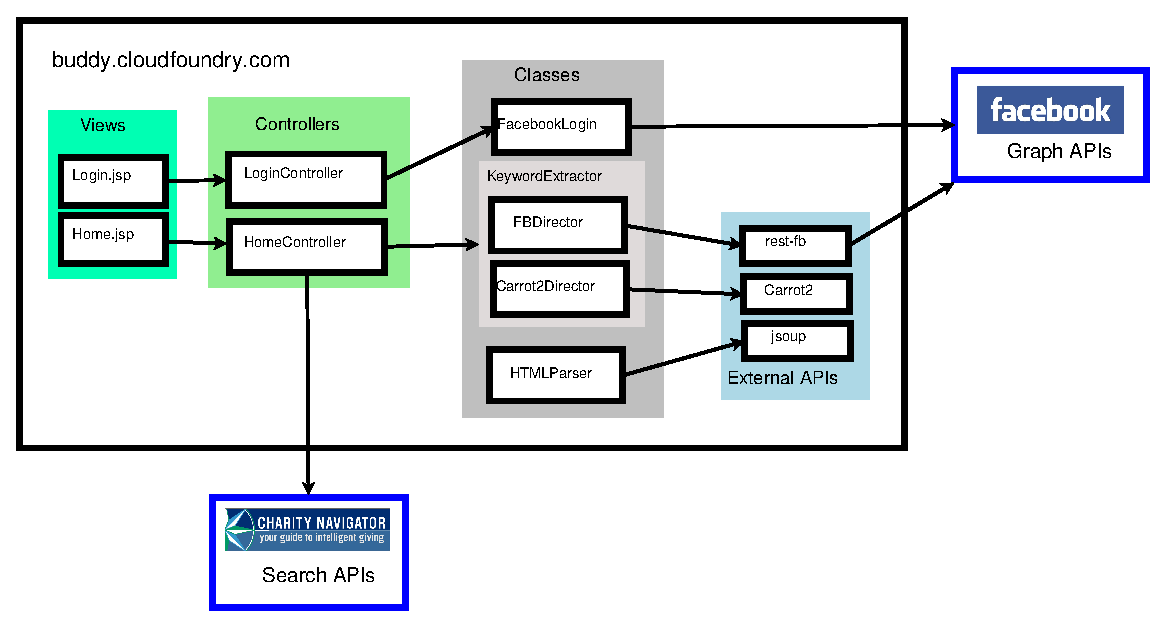
\includegraphics[width=6.5in]{./figures/arch-diagram.eps}
\caption{Architecture Overview}\label{fig:arch}
\end{figure}


\section{The App Maintenance}
The App is currently being maintained by Duy Nguyen(nguyend@vmware.com), Feng Ji(jif@vmware.com), Zhichao Li(zhichaoli@vmware.com), and Moussa Ehsan(ehsanm@vmware.com). You can contact them for further information or to report any bugs.

\section{Future Work}
There are several "nice-to-have" todoes that could go beyond the two weeks' limitation.  First, we would like to make data mining part more accurate and bug free to display.  Second, it would be nice to have a mobile App as the client of buddy.cloudfoundry.com. Third, it would be nice to store feedback from the community on the quality of the charity organizations so that we maintain history records of the charity programs and update the match results to benefit the community in a better way. 

%\bibliographystyle{unsrt}
%\bibliography{anonymous,zk,foursquare,wormhole}

\end{document}
